\documentclass[12pt,a4paper]{article}
\usepackage[utf8]{inputenc}
\usepackage[T1]{fontenc}
\usepackage{textcomp}
\usepackage{amsmath}
\usepackage{amsfonts}
\usepackage[francais]{babel}
\usepackage{amssymb}
\usepackage{graphicx}
\usepackage[top=2.00cm]{geometry}
\usepackage{enumitem}
%\usepackage{mathtools}
\usepackage{bigcenter}
\usepackage{multicol}
%\usepackage{minibox}

%Modif des enumerates numeros en gras. leftmargin=*,
\setlist[enumerate]{label=\textbf{\arabic*}.}

\usepackage{titlesec}
%modif des titres de section diminuer la taille
\renewcommand{\thesection}{\Roman{section}}
\titleformat{\section}
  {\normalfont\Large\bfseries\scshape}{\thesection}{1em}{}
\titleformat{\subsection}
  {\normalfont\large\bfseries}{\thesubsection}{1em}{}

\author{CHARNAY Valentin, FINOT Sylvain}
\title{
\includegraphics[scale=0.3]{logousmb}\\
Compte rendu de TP : \\ \scshape Ondes Centimétriques}
\date{1 Février 2017}
\begin{document}
	\maketitle
	\rule{\linewidth}{0.4pt}
	\section{Antenne cornet}
	\subsection{Nature et polarisation de l'onde}
	Dans cette partie, on souhaite déterminer la nature de l'onde émise par l'antenne cornet (constituée d'une diode Gunn). Pour ce faire, nous plaçons une antenne réceptrice a une distance "d" variable et nous mesurons la tension "A" (continue) à ses bornes à l'aide d'un oscilloscope.\\
	On trace par la suite
	$$\ln A = f(\ln D)$$
	\begin{bigcenter}
		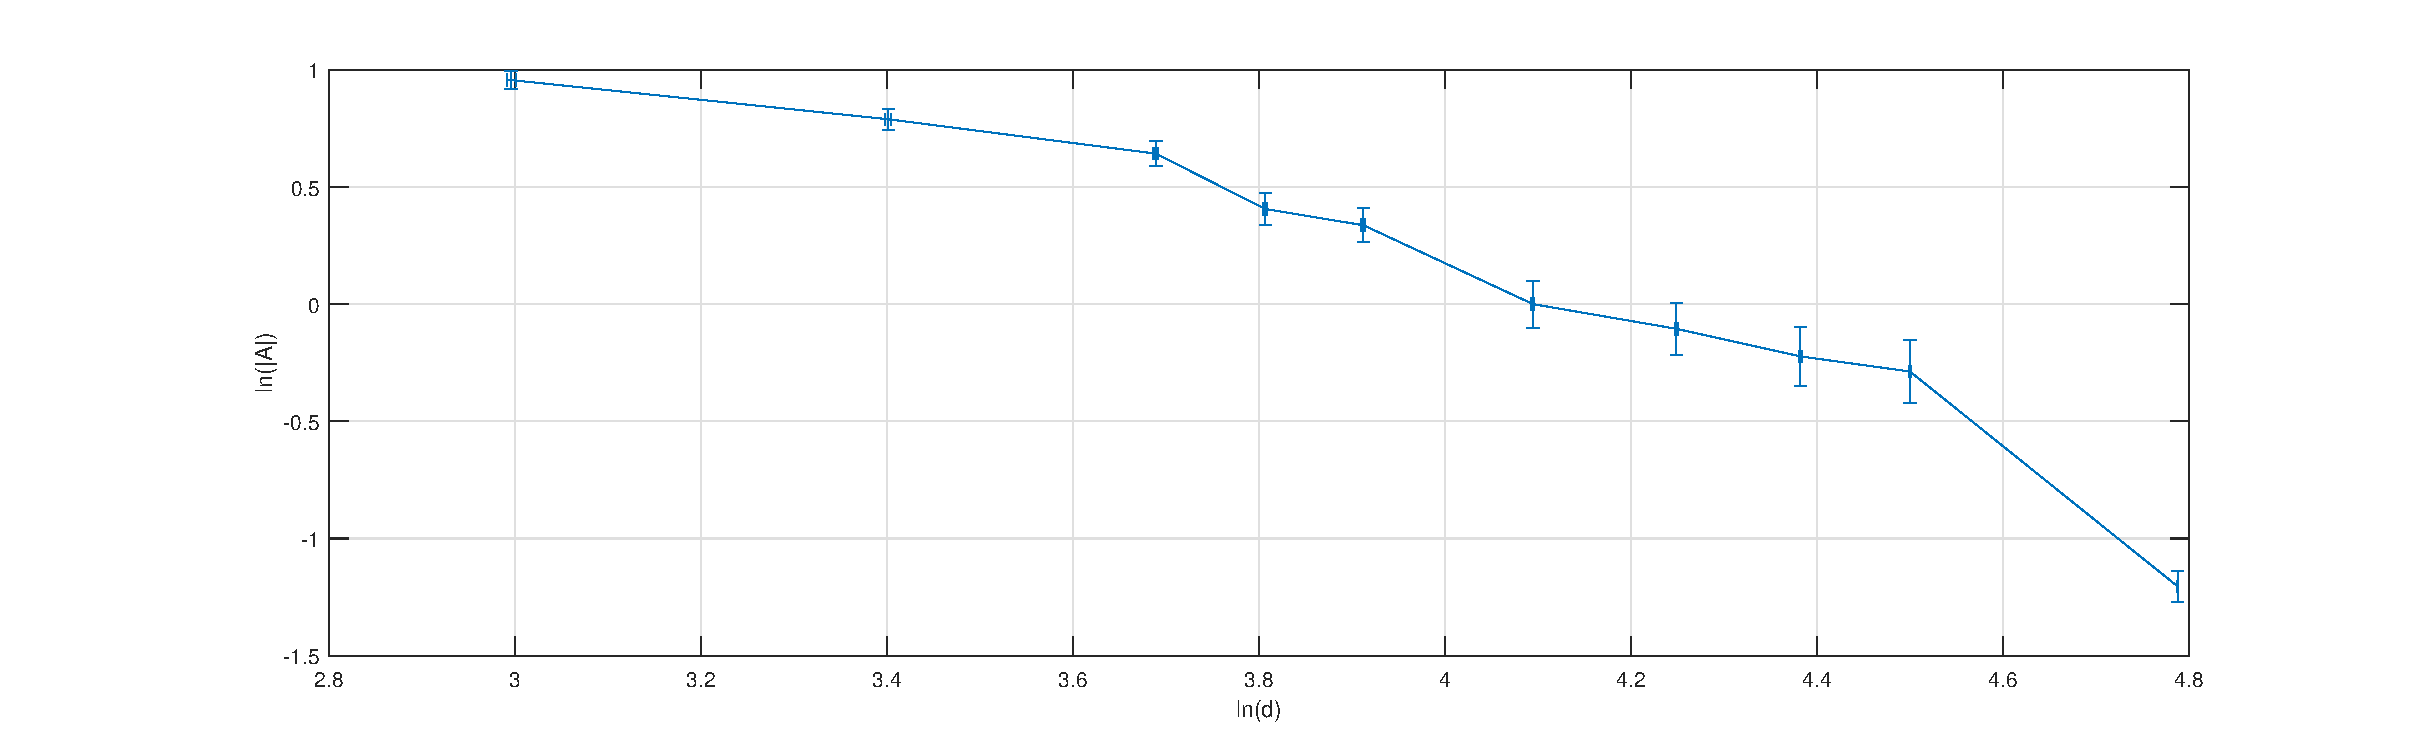
\includegraphics[scale=0.5]{matlab/lnA}
	\end{bigcenter}
	On remarque que la tension aux bornes de l'antenne diminue en l'éloignant de l'émetteur, on peut donc en conclure que les ondes émises ne sont pas des ondes planes. On en déduit donc qu'il s'agit d'une onde sphérique, mais concentrée par le cornet. Les barres d'erreur du graphe ci-dessus sont calculées à partir d'incertitudes de lectures. On estime que les incertitudes sont de l'ordre de la plus petite graduation, on néglige les éventuelles fluctuations de la tension A. Ainsi $\Delta d$ vaut 1 mm et $\Delta A$ vaut (1/5) du calibre de l'oscilloscope.
	Afin de déterminer une éventuelle polarisation de l'onde, il suffit de faire pivoter l'antenne par rapport à l'axe "Émetteur-Récepteur". On remarque alors qu'après rotation de 90° (i.e l'antenne parallèle au sol), la tension est nulle, ce qui implique que l'onde est polarisée.
	\subsection{Diagramme de rayonnement}
	On s'intéresse maintenant au diagramme de rayonnement de l'antenne.\\
	On effectue dans un premier un temps un relevé de $A(\psi)$. Sans réelle surprise, on remarque que $A$ est maximale pour $\psi=90$°. On normalise l'expression (facultatif) en posant \~{A}$\equiv\dfrac{A(\psi)}{A_{max}}$. Enfin, on trace \~{A} en coordonnées polaires.\\
\begin{figure}[h]
	\centering
	\caption[Diagramme de rayonnement]{Diagramme de rayonnement}
	\label{fig:rayonnement}
	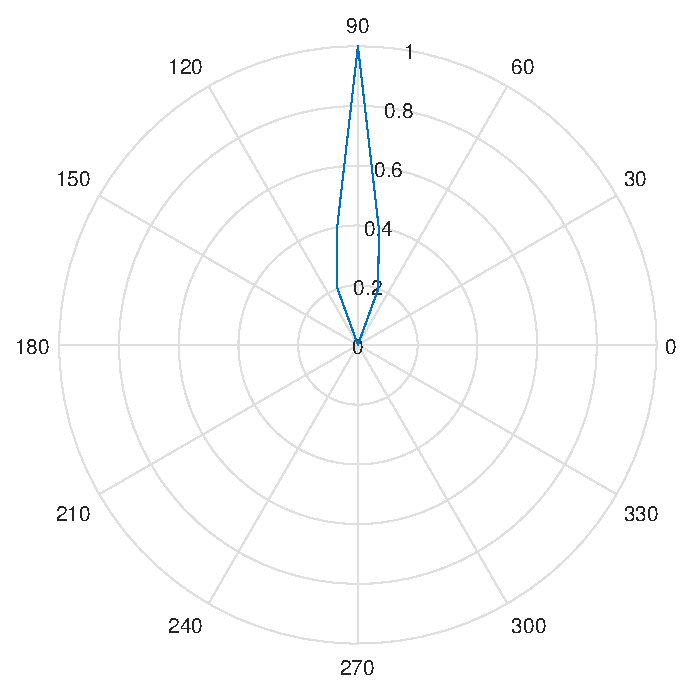
\includegraphics[scale=0.6]{matlab/Rayonnement}
\end{figure}

	
	\section{Ondes centimétriques libres}
	\subsection{Ondes stationnaires}
	En plaçant une plaque métallique face au cornet à une distance d'environs 20cm, celui-ci agit comme un miroir. Il s'établit alors un régime d'ondes stationnaires entre le cornet et la plaque métallique (superposition de l'onde incidente et de l'onde réfléchie). En déplaçant l'antenne réceptrice entre le cornet et la plaque, on observe une série de maxima et de minima. La distance entre deux maximums successifs est $\lambda$/2 où $\lambda$ est la longueur d'onde des ondes centimétriques. On relève quelques points:
	\begin{center}
		\begin{tabular}{|c|c|}
			\hline 
			Maximum n° & d (cm) \\ 
			\hline 
			1 & 15 \\ 
			\hline 
			2 & 13.25 \\ 
			\hline 
			3 & 11.75 \\ 
			\hline 
			4 & 10 \\ 
			\hline 
			5 & 6.7 \\ 
			\hline 
		\end{tabular} 
	\end{center}
	Pour plus de précision, on calcule en prenant 5 maximums : 
	\setlength\columnseprule{0.5pt}
	\begin{multicols}{2}
		\begin{align*}
		15-6,7 &= \dfrac{5\lambda}{2}\\
		\implies \lambda &= \dfrac{2(15-6,7)}{5}=3,32 \text{ cm}
		\end{align*}
		\vfill
		\columnbreak
		\begin{align*}
		\Delta \lambda &= \sqrt {\left( \Delta d_{1}\right) ^{2}+\left( \Delta d_{2}\right) ^{2}}\\
		\implies \Delta \lambda &= \sqrt {0,1^2+0,1^2}=0,14 \text{ cm}
		\end{align*}
	\end{multicols}
	$$\lambda = 3,32\pm1,4.10^{-1} \text{cm}$$
	Comparons ce résultat aux données constructeur : Fréquence d'émission 9,35GHz.
	\begin{align*}
	c &= \lambda.\nu\\
	\iff \lambda &= \dfrac{c}{\nu}\\
	&=\dfrac{c}{9,35.10^9}\\
	&=3,2 \text{ cm}
	\end{align*}
	Le résultat expérimental correspond bien aux données fournies par le constructeur. 
	
	\subsection{Interféromètre de Michelson}
	
	Nous effectuons l'expérience suivante :
	\begin{multicols}{2}
		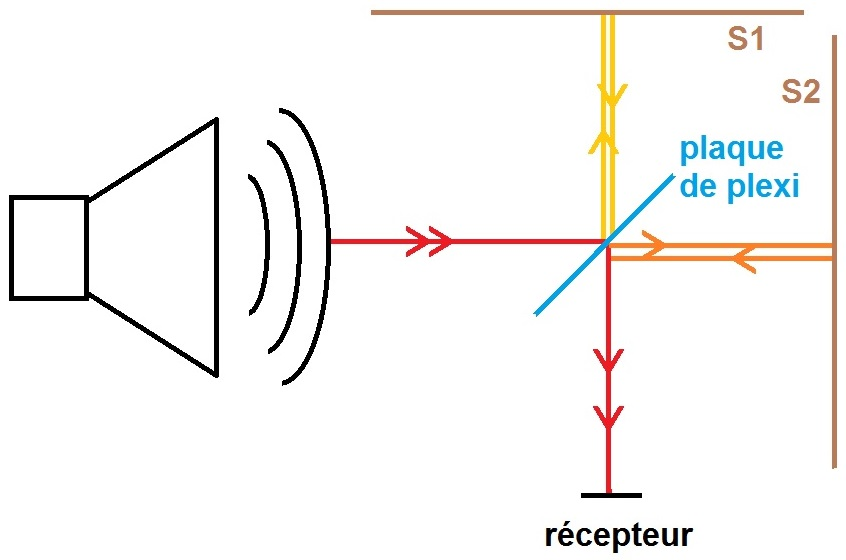
\includegraphics[scale=0.3]{schem1}
		\columnbreak
		
		Nous envoyons un signal sur une plaque de plexiglas. Une partie du signal est réfléchie (jaune), l'autre la traverse (orange. Au final les deux parties se rejoignent (rouge) et sont captées par le récepteur.
	\end{multicols}
	Bien évidemment, en tenant compte du chemin parcouru par les deux signaux, nous observons un décalage. Avec une distance d'environ 20 cm entre les différents objets, nous avons donc une interférence observée sur l'oscilloscope. Nous faisons varier la distance entre la plaque de plexiglas et la source, nous avons obtenu un premier maximum à 30 cm et un $5^e$ maximum à 38.5 cm.
	
	On a alors : 
	$$\lambda = \frac{2}{5}.\Delta d$$
	$$AN :\hspace{0.2cm} \lambda \approx \frac{2}{5}( 38.5 - 30) \approx 3.4 \hspace{0.2cm} cm$$
	On trouve alors une longueur d'onde d'environ 3.4 cm ce qui avec les incertitudes visuelles dans les mesures de la distance est correct (3.2 cm théoriquement).
	
	\subsection{Interférences par les fentes de Young}
	Nous devions réaliser l'expérience suivante (pas mené a son terme) :
	\begin{multicols}{2}
		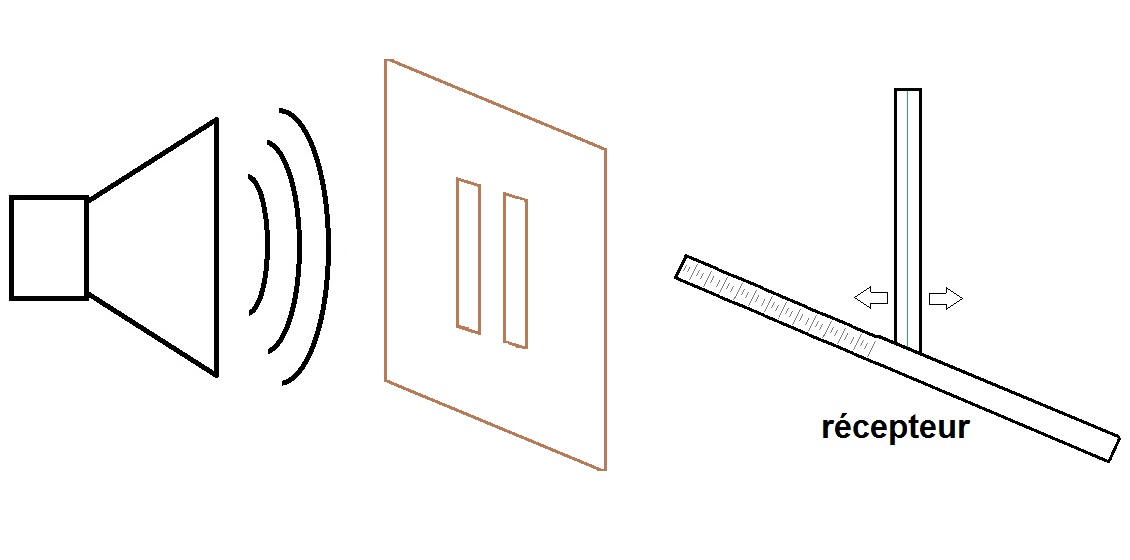
\includegraphics[scale=0.28]{schem2} 
		\columnbreak
		
		Le principe est simple : la taille de la fente étant de l'ordre du centimètre (ordre de grandeur de la longueur d'onde utilisé) on voit apparaitre le phénomène de diffraction au niveau des fentes. Les deux "nouvelles" ondes vont alors créer une interférence que l'on visualisera par des maximums et des minimums avec l'oscilloscope relié au récepteur. 
	\end{multicols}
	En effectuant des mesures de la distance entre les interfranges, nous serions en mesure déterminer la longueur d'onde de notre signal.\\
	On rappel  que : $i=\dfrac{\lambda D}{a}$ où a est la distance séparant les deux fentes et D la distance entre les fentes et la position (écran dans le visible) où l'on observe les fentes.\\
	Dans notre cas l'interfrange est trop grand pour pouvoir être mesuré correctement avec le matériel disponible. ($i=\dfrac{3,2*D}{0,9}\approx1,33m$)
	\begin{center}
		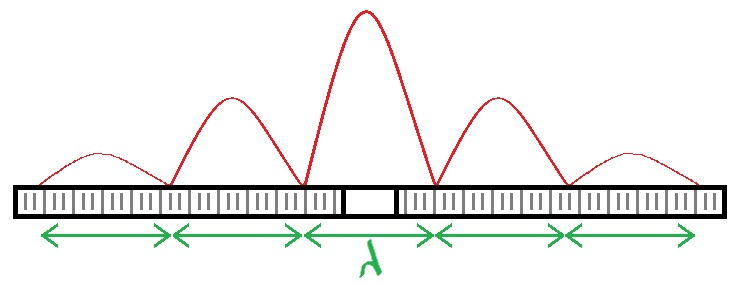
\includegraphics[scale=0.6]{schem3} 
	\end{center}
	En récoltant un grand nombre de maximum (ce qui pose problème ici), nous serions en mesure de trouver un résultat relativement précis et de retrouver une longueur d'onde d'environ 3.2 cm.
	\subsection{Diffraction des ondes centimétriques}
	\begin{itemize}[label=$\circ$]
		\item Dans cette expérience, on réalise la même chose que précédemment en utilisant cette fois-ci une plaque trouée d'un diamètre de 1 cm. Par faute de temps, nous n'avons pu effectuer cette manipulation, mais le résultat est bien connu. 
		
		S'agissant d'une onde, celle-ci possède la propriété de diffraction (comme précédemment) et le résultat obtenu est cette fois la réémission de l'onde orientée comme la fente (ici de manière sphérique).
		
		\item En faisant "cogner" l'onde sur le bord de la plaque, théoriquement nous aurions dû obtenir un signal identique comme le montre le schéma suivant. C'est grâce à cette propriété que nous pouvons écouter la radio (ondes centimétriques) quasiment partout. 
		\begin{center}
			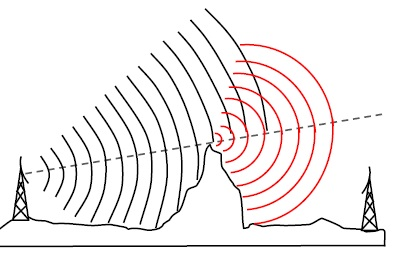
\includegraphics[scale=0.5]{schem4}
			
		\end{center}
	\end{itemize} 
	\begin{quotation}
		\textit{"The black holes of nature are the most perfect macroscopic objects there are in the universe: the only elements in their construction are our concepts of space and time."} Subrahmanyan CHANDRASEKHAR
	\end{quotation}
	
\end{document}
